%!TEX root = ../report.tex
\documentclass[report.tex]{subfiles}
\begin{document}
\chapter{Evaluation and results}
In this research and development project, three experiements are being conducted with respected to three use cases: (1) Grasp object by sliding motion along surface and (2) Perform writing task and (3)Resting elbow manipulation. First, the set up of the experiements will be introduce. Second,the experiments/evaluation you are performing to analyse the use case will be described. At last, the results of the experiments will be delievered. In this chapter, the experiements and evaluation will be divided according to use cases.
    \section{Setup}
    The three experiement setups in this research and development project are the same but with different intial position.
    The tool and robot that is being use inthe experiements are listed below:
    \begin{itemize}
        \item Kinova® Gen3 Ultra lightweight robot maniputlator is attached to a table
        \item A Robotiq 2F-85 gripper is attached to the 7th joint of the Kinova arm
        \item The Kinova arm is connect to a laptop with LAN cable
        \item A Xbox controller
    \end{itemize}
    The direction that discuss in this chapter in according to the tool frame, which is equals to the task frame, robot base frame and the world frame.

    \section{Use case 1 - Grasp object by sliding motion along surface}
    \paragraph{\larger{Experiment design}\\}
    The objective of this case study is to achieve a successful object grasp by sliding the robot manipulator along a contact surface, serving as a proof-of-concept task to set up the necessary infrastructure for task execution. It is assumed that the pose of the object is already known, and the only item present on the table is the object to be grasped, with no obstacles in the way. The contact surface is also well-defined.

    The manipulation process begins with the manipulator approaching the contact surface, such as a table with the target object placed upon it. As the manipulator hovers above the contact surface, it proceeds to advance towards it until physical contact is established. By activly monitoring the velocity along linear Z axis $v_{lin_z}$in world frame. If the absolute value of $v_{lin_z}$ for 10 samples is less than a threshold value. The contact between a surface and the robot manipulator is being established.
    After contact is established, the manipulator slides along the linear x direction for 10 cm $d_{x} = 0.1$ until it reaches a grasping region. Finally, the end-effector performs a grasping motion.
    
    In the evaluation, first, we will assess the power consumption of all the joints during motion in both contact and contactless scenarios. The goal is to determine whether performing the task on a contact surface leads to an increase in energy efficiency. Since the voltage and current of each joint are being logged during each trial,by using $P_i = V_i A_i$, where $P_i$ is the power consumption, $V_i$ is the voltage and $A_i$ is the current of a particular joint respectively, we can calculate the power consumption of each joint.

    Second, we will analyze the joint torque $\tau_{Ji}$ for each joint to determine whether the joint torque decreases when contact is established. Where $\tau_J$ indicate joint torque and $i$ is the joint number.

    The hypothesis for use case 1 posits that in the contact scenario, energy efficiency will be elevated while joint torque will experience a reduction.

    \begin{figure}[H]
        \captionsetup[subfigure]{justification=centering}
        \begin{subfigure}{0.49\textwidth}
                \centering
                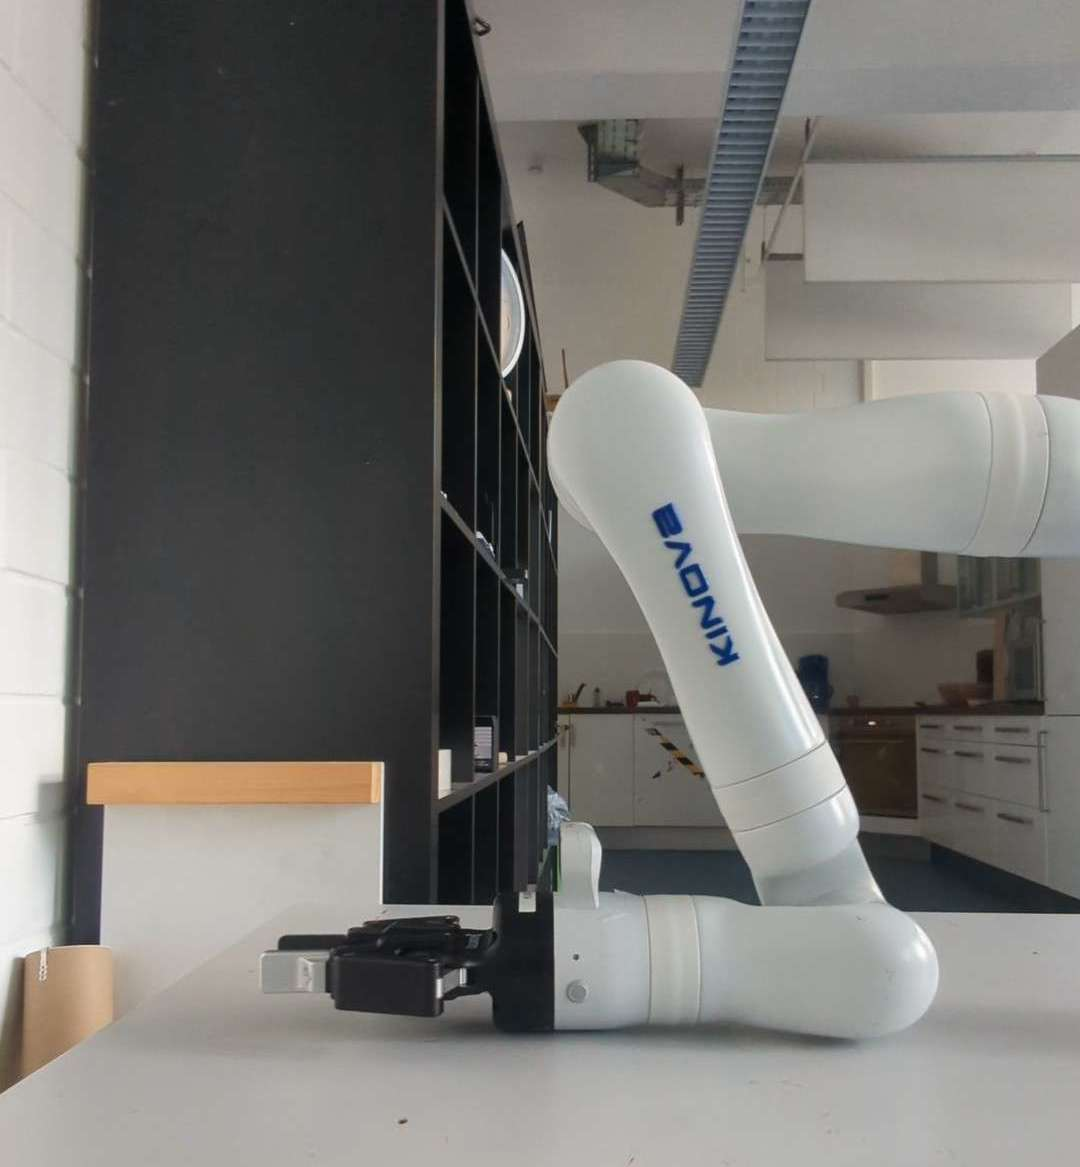
\includegraphics[width=\linewidth]{images/us1_contact2.jpg}
                \caption{The moment when the contact established. The robot moves from the initial position until contact is established}
                \label{fig:us1_con}
            \end{subfigure}
            \begin{subfigure}{0.49\textwidth}
                \centering
                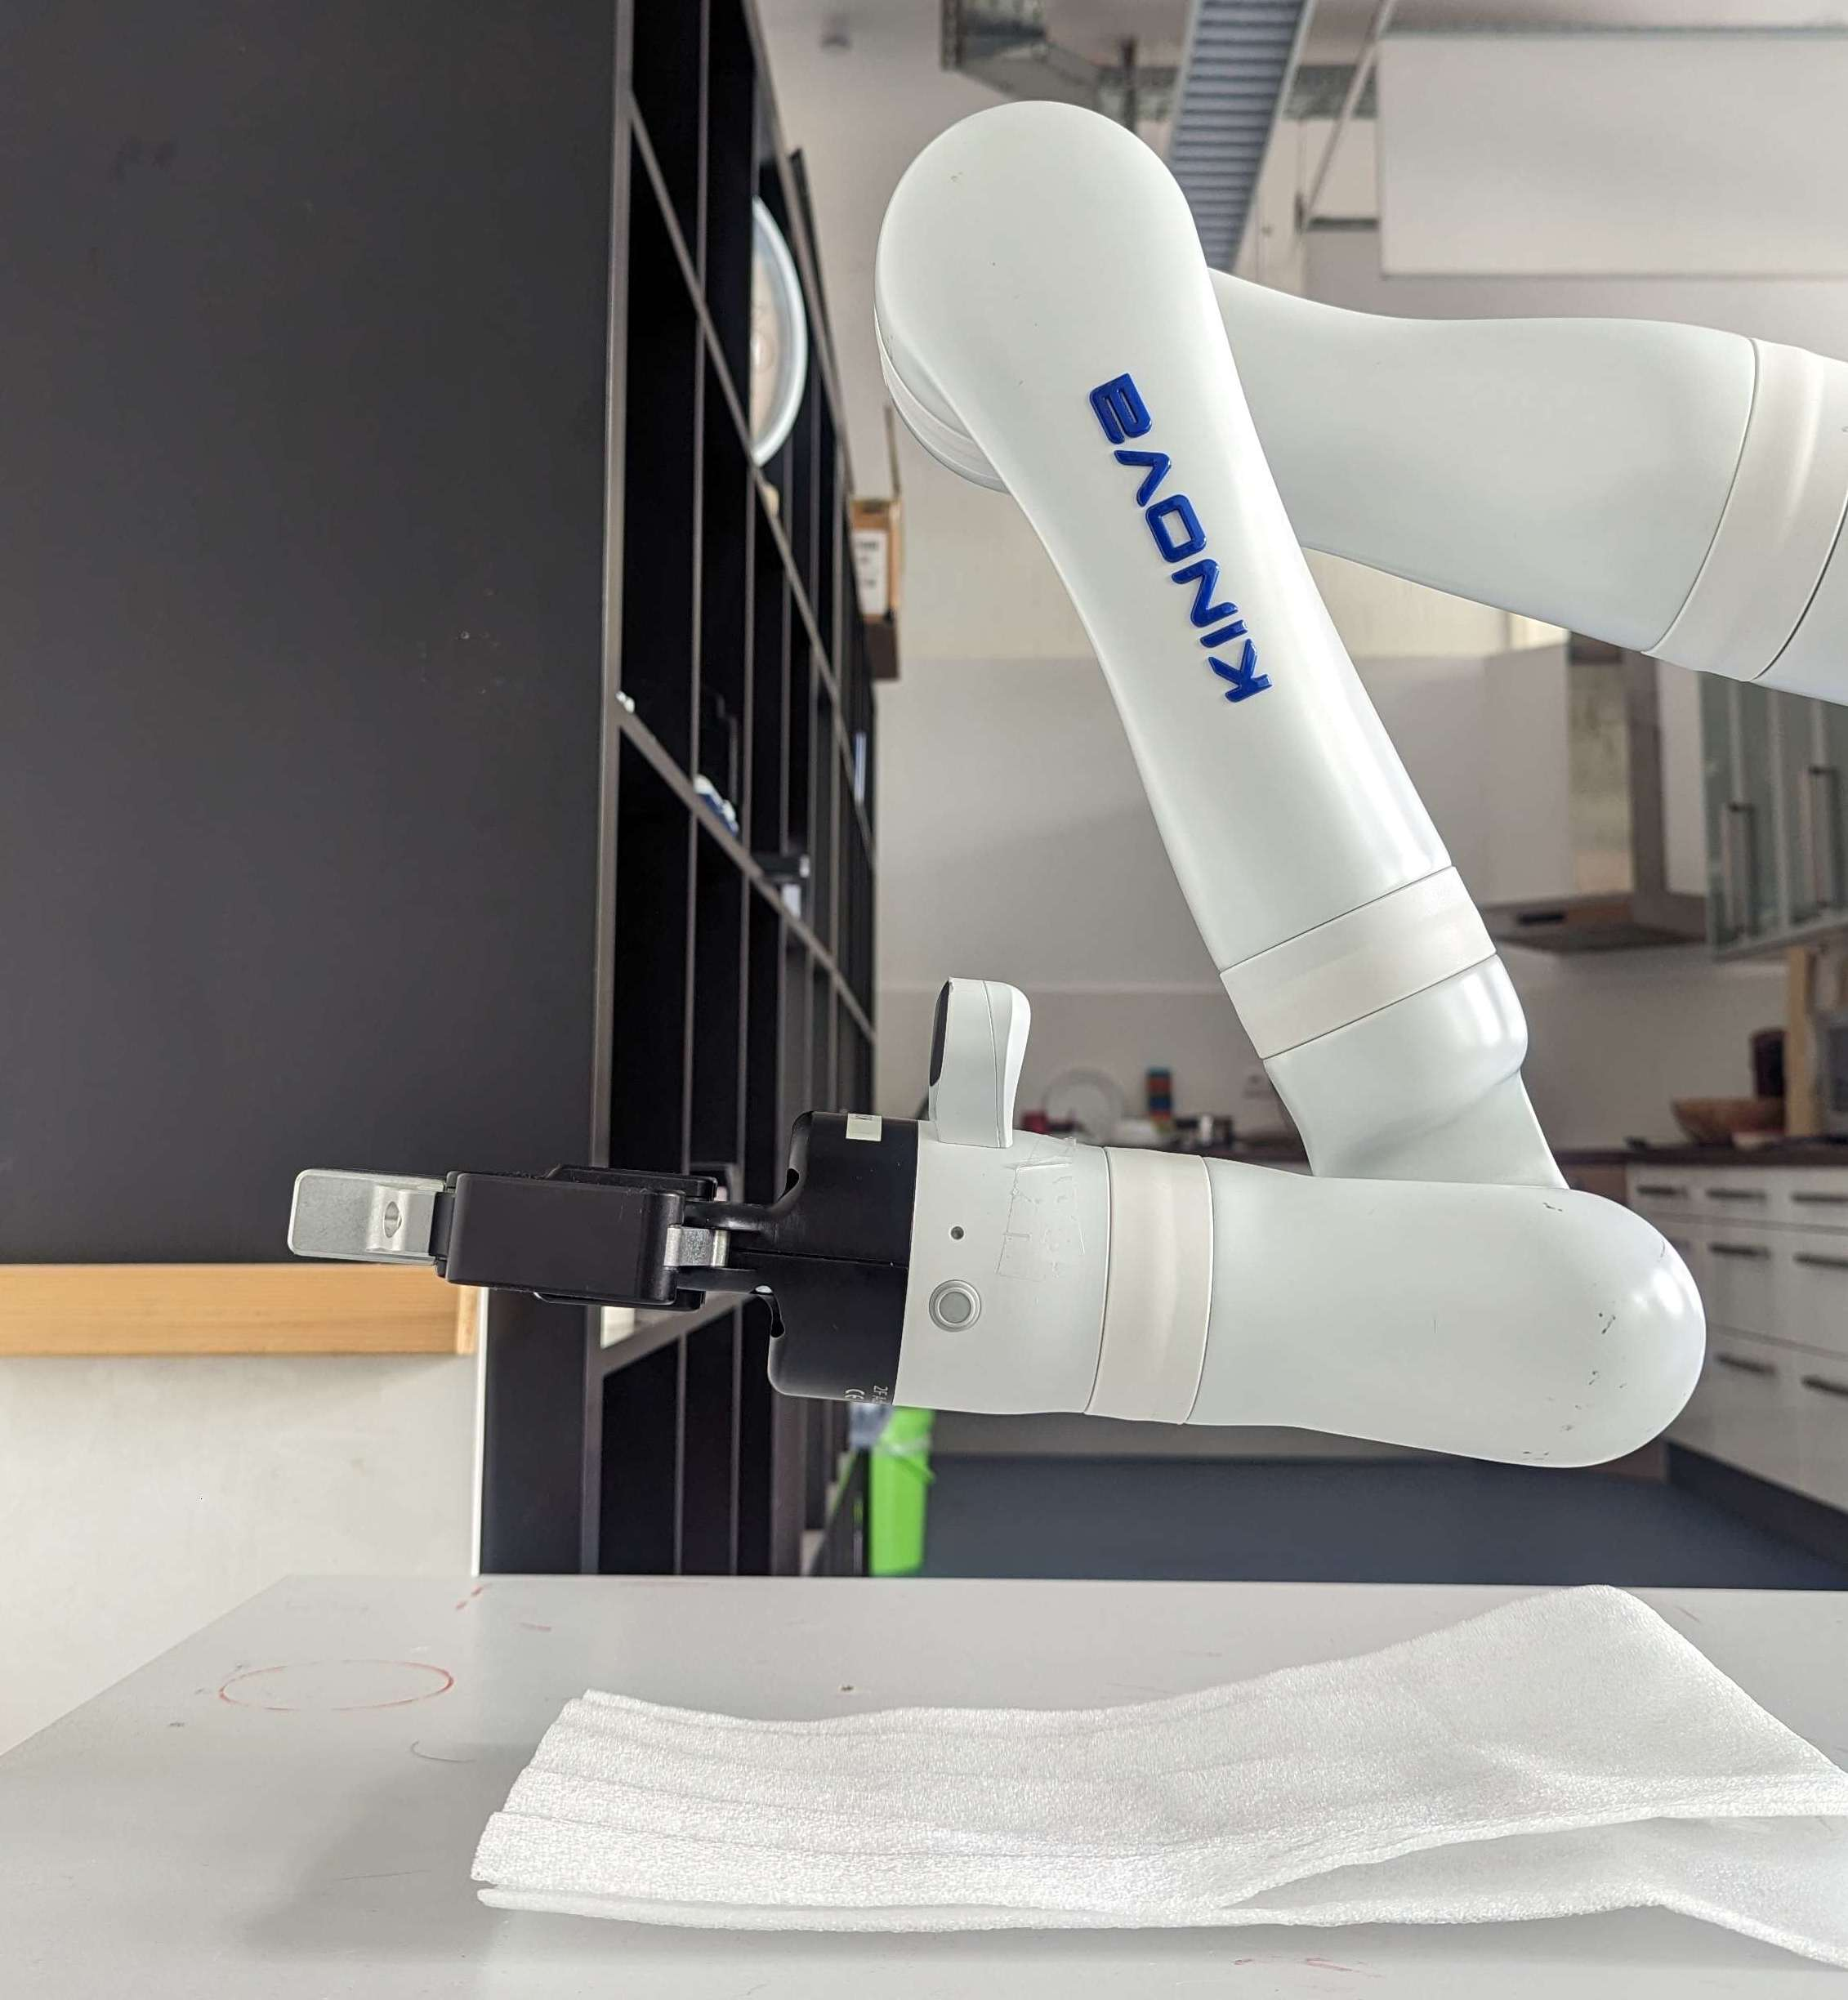
\includegraphics[width=\linewidth]{images/us1_contactless.jpg}
                \caption{The moment before the robot move along linear X direction. The robot arm moves along Z direction for 25 cm from the initial position}
                \label{fig:us1_nocon}
            \end{subfigure}
            \caption{The robot pose before it move forward}
        \end{figure}
    \paragraph{\large{Setup}\\}
    Figure \ref{fig:us1_init} shows the initial pose of the robot arm of use case 1. To ensure that the robot consistently begins each trial run from its precise starting position, it is necessary to press the B button on the Xbox controller. The motion will starts at a fixed starting pose $q = \{6.28318,0.261895,3.14159,4.01417,0,\\0.959856,0.57079\}$ in radian.
    \begin{figure}[H]
        \centering
        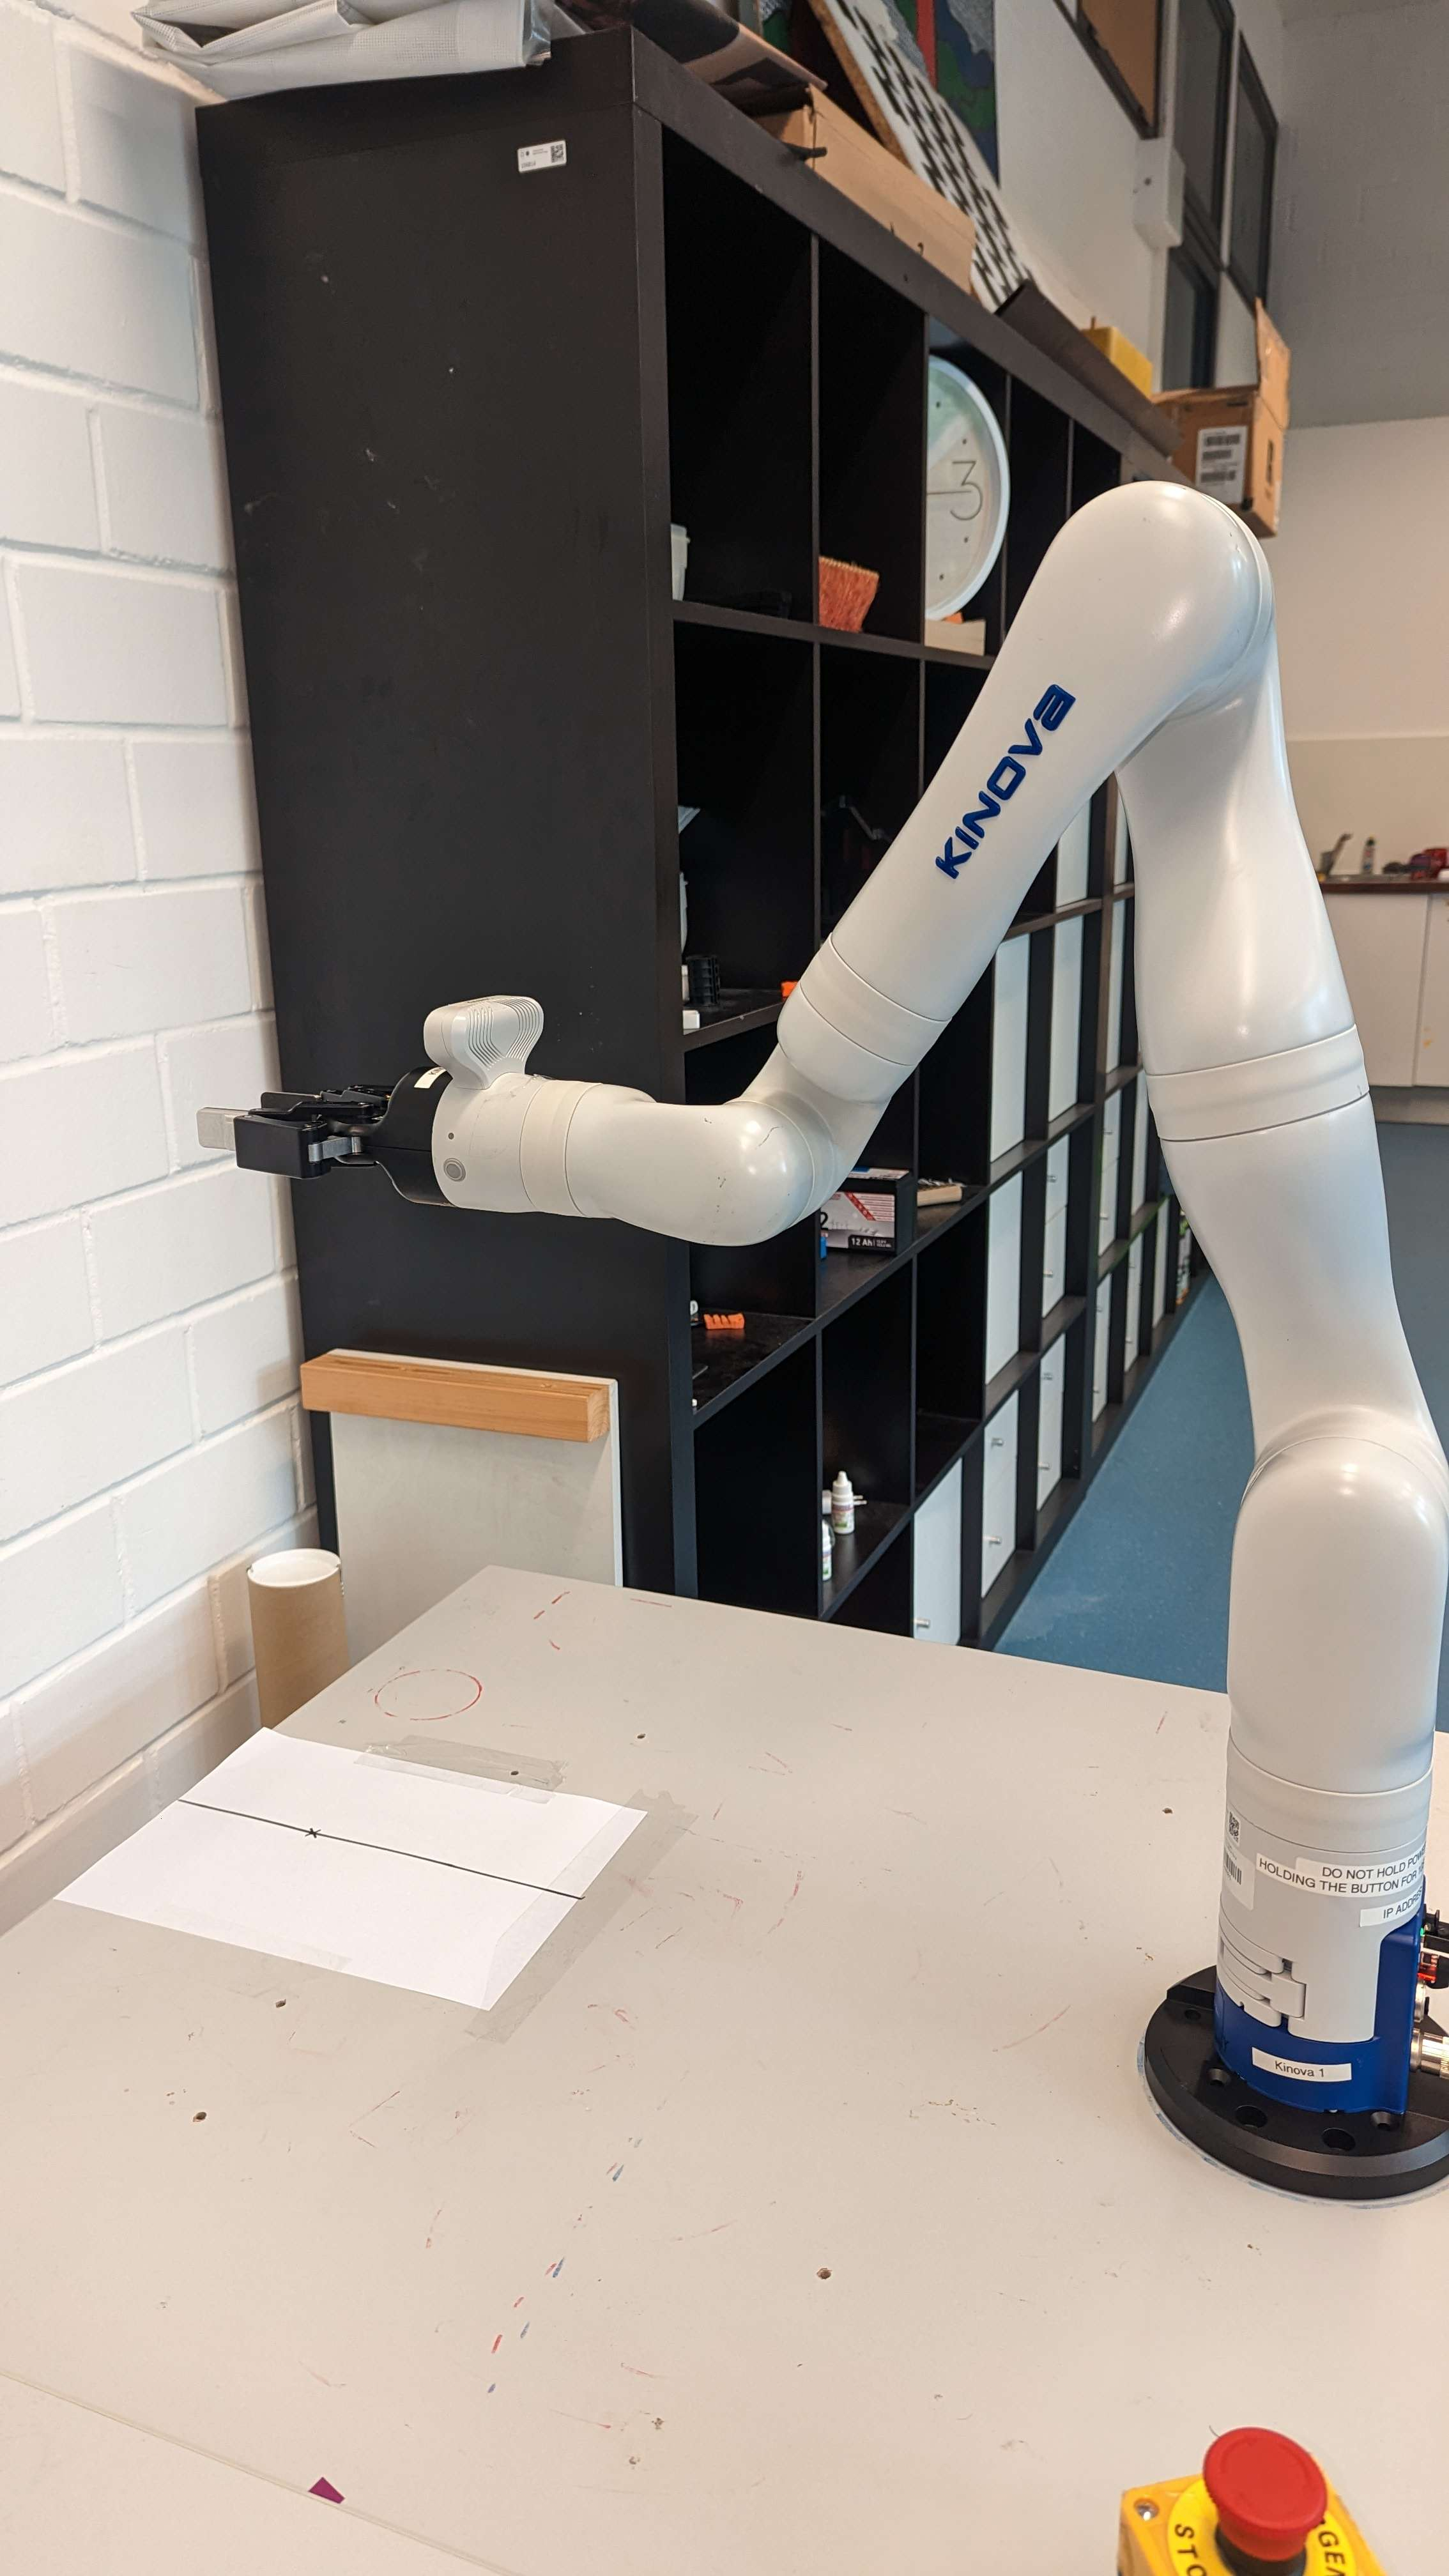
\includegraphics[width=0.4\linewidth]{images/us1_initial.jpg}
        \caption{The initial pose of the robot arm of use case 1}
        \label{fig:us1_init}
    \end{figure}
    \paragraph{\large{Evaluation}\\}
    Table \ref{tab:us1_table_power} presents the average voltage, current, and power consumption for each joint in both contact and contactless scenarios. Interestingly, the average voltage remains nearly unchanged across both scenarios. However, a notable observation arises when comparing the average current and power consumption among the joints.

    Specifically, joints 1, 3, and 5 exhibit a substantial requirement for power and current. This phenomenon can be attributed to the robot's motion, which involves movement along the linear z-direction while maintaining a fixed z-position to prevent the collapse of the robot arm. When comparing the average current and power consumption between the two scenarios for individual joints, joint 1 and 5 experience significant increases of 68.2\% and 90.6\%, respectively. This increase is likely a result of the robot's need to maintain the end effector's position mid-air during movement along the linear x-direction towards the grasping position.
    
    Furthermore, joint 3 stands out as its power consumption in the contact case is 40.5\% higher than in the contactless case. This discrepancy may be attributed to the increased power required for this joint to move the end effector along the linear x-direction while overcoming friction with the contact surface.
    
    Examining the average joint torque individually, as shown in Table \ref{tab:us1_table_torque}, reveals that the torque on joints 1 and 5 increases by 41.2\% and 47.5\%, respectively, in the contactless case. In contrast, joint 3 experiences a 55.8\% decrease in torque under contactless conditions. However, when considering the average torque across all joints, the contact case exhibits an average torque of 1.9857 N, while the contactless case surprisingly records a lower average torque of 0.8256 N.
    
    From the analysis of this data, it becomes evident that performing the task on a contact surface can lead to increased energy efficiency in specific joints, such as the shoulder joint (joint 1) and wrist joint (joint 5). There is also the possibility that the energy efficiency of the elbow joint increases, given the increase in joint torque under contact conditions, likely due to the need to overcome friction with the contact surface. Further studies can explore this behavior with different contact surfaces featuring varying textures.

\begin{table}[H]
    \centering
    \resizebox{\textwidth}{!}{%
    \begin{tabular}{c|ccc|ccc|}
    \cline{2-7}
    \multicolumn{1}{l|}{}       & \multicolumn{3}{c|}{Contact}                                                                                                                                                                                                                     & \multicolumn{3}{c|}{Contactless}                                                                                                                                                                                                                 \\ \hline
    \multicolumn{1}{|c|}{Joint} & \multicolumn{1}{c|}{\begin{tabular}[c]{@{}c@{}}Average\\ voltage (V)\end{tabular}} & \multicolumn{1}{c|}{\begin{tabular}[c]{@{}c@{}}Average\\ current (A)\end{tabular}} & \begin{tabular}[c]{@{}c@{}}Average\\ power consumption(W)\end{tabular} & \multicolumn{1}{c|}{\begin{tabular}[c]{@{}c@{}}Average\\ voltage (V)\end{tabular}} & \multicolumn{1}{c|}{\begin{tabular}[c]{@{}c@{}}Average\\ current (A)\end{tabular}} & \begin{tabular}[c]{@{}c@{}}Average\\ power consumption(W)\end{tabular} \\ \hline
    \multicolumn{1}{|c|}{0}     & \multicolumn{1}{c|}{23.4669}                                                       & \multicolumn{1}{c|}{0.1283}                                                        & 3.0093                                                                 & \multicolumn{1}{c|}{23.4727}                                                       & \multicolumn{1}{c|}{-0.0416}                                                       & -0.9776                                                                \\ \hline
    \multicolumn{1}{|c|}{1}     & \multicolumn{1}{c|}{23.3939}                                                       & \multicolumn{1}{c|}{-0.7882}                                                       & -18.4433                                                               & \multicolumn{1}{c|}{23.3541}                                                       & \multicolumn{1}{c|}{-1.3291}                                                       & -31.0272                                                               \\ \hline
    \multicolumn{1}{|c|}{2}     & \multicolumn{1}{c|}{3.1786}                                                        & \multicolumn{1}{c|}{0.0626}                                                        & 1.4536                                                                 & \multicolumn{1}{c|}{23.1764}                                                       & \multicolumn{1}{c|}{0.0104}                                                        & 0.2443                                                                 \\ \hline
    \multicolumn{1}{|c|}{3}     & \multicolumn{1}{c|}{23.2972}                                                       & \multicolumn{1}{c|}{0.5766}                                                        & 13.4307                                                                & \multicolumn{1}{c|}{23.2945}                                                       & \multicolumn{1}{c|}{0.3427}                                                        & 7.9853                                                                 \\ \hline
    \multicolumn{1}{|c|}{4}     & \multicolumn{1}{c|}{23.3074}                                                       & \multicolumn{1}{c|}{0.1844}                                                        & 4.2983                                                                 & \multicolumn{1}{c|}{23.2133}                                                       & \multicolumn{1}{c|}{0.0976}                                                        & 2.2659                                                                 \\ \hline
    \multicolumn{1}{|c|}{5}     & \multicolumn{1}{c|}{23.2875}                                                       & \multicolumn{1}{c|}{0.2210}                                                        & 5.1487                                                                 & \multicolumn{1}{c|}{23.2839}                                                       & \multicolumn{1}{c|}{0.4215}                                                        & 9.8156                                                                 \\ \hline
    \multicolumn{1}{|c|}{6}     & \multicolumn{1}{c|}{23.1337}                                                       & \multicolumn{1}{c|}{-0.0084}                                                       & -0.1950                                                                & \multicolumn{1}{c|}{23.1356}                                                       & \multicolumn{1}{c|}{-0.0129}                                                       & 0.2994                                                                 \\ \hline
    \end{tabular}%
    }
    \caption{Table of the average voltage, current and power consumption of each joint in contact and contactless case}
    \label{tab:us1_table_power}
    \end{table}
\begin{table}[H]
    \centering
    % \resizebox{0.5\textwidth}{!}{%
    \begin{tabular}{c|c|c|}
    \cline{2-3}
    \multicolumn{1}{l|}{}       & Contact                                                      & Contactless                                                  \\ \hline
    \multicolumn{1}{|c|}{Joint} & \begin{tabular}[c]{@{}c@{}}average\\ torque (N)\end{tabular} & \begin{tabular}[c]{@{}c@{}}average\\ torque (N)\end{tabular} \\ \hline
    \multicolumn{1}{|c|}{0}     & 0.2164                                                       & -0.1564                                                      \\ \hline
    \multicolumn{1}{|c|}{1}     & 9.8474                                                       & 16.7563                                                      \\ \hline
    \multicolumn{1}{|c|}{2}     & 0.3025                                                       & 0.9884                                                       \\ \hline
    \multicolumn{1}{|c|}{3}     & -3.1071                                                      & -1.3727                                                      \\ \hline
    \multicolumn{1}{|c|}{4}     & 0.3014                                                       & 0.3063                                                       \\ \hline
    \multicolumn{1}{|c|}{5}     & -1.7027                                                      & -2.5120                                                      \\ \hline
    \multicolumn{1}{|c|}{6}     & -0.0787                                                      & -0.1095                                                      \\ \hline
    \end{tabular}%
    % }
    \caption{Table of the average torque of each joint in contact and contactless case}
    \label{tab:us1_table_torque}
    \end{table}
    \newpage
    \section{Use case 2 - Perform writing task}
    \paragraph{\larger{Experiment design}\\}
    The objective of use case 2 is to replicate the act of drawing a line on paper, emulating human writing. To commence the manipulation task, the gripper securely holds the pen or marker. Since this use case focus on the study of if the motion is accurate when robot exploits the contact surface, the motion starts when the marker pen makes contact with the reference starting on as figure \ref{fig:us2_pen} shows.Upon achieving contact, the robot follows a predefined motion pattern to draw a line which the robot arm moves along linear x direction for 10 cm.
    The evaluation will involve comparing the trajectory with and without contact between the robot and the supporting surface. We define accuracy as the maxiumn displacement in linear y direction between a drawn trajectory and the pre-define straight line on the paper.
    
    The hypothesis for use case 2 suggests that in the contact scenario, accuracy will be enhanced, and the trajectory will exhibit greater stability.
    \raggedbottom
    \paragraph{\large{Setup}\\}
    Considering that the purpose of this use case is to perform a writing task, it's important to note that, similar to human writing, the writing motion does not commence from mid-air initially. Instead, the writing task initiates when the tip of the marker pen makes contact with a designated starting reference point on the paper as figure \ref{fig:us2_pen} demostrates. In this particular use case, we will conduct two experiments. In the first experiment, we will establish contact before proceeding with the writing task, whereas in the second experiment, no contact will be established beforehand. Figure \ref{fig:us2_init_con} and \ref{fig:us2_init_nocon} show the initial set up of both experiements at side view. In \ref{fig:us2_init_nocon}, The ruler indicates that the distance from the center of the gripper to the table surface is 10 cm. This measurement serves as the initial height for the writing motion in situations where there is no physical contact with the table.
    \begin{figure}[H]
        \centering
        \captionsetup[figure]{justification=centering}
        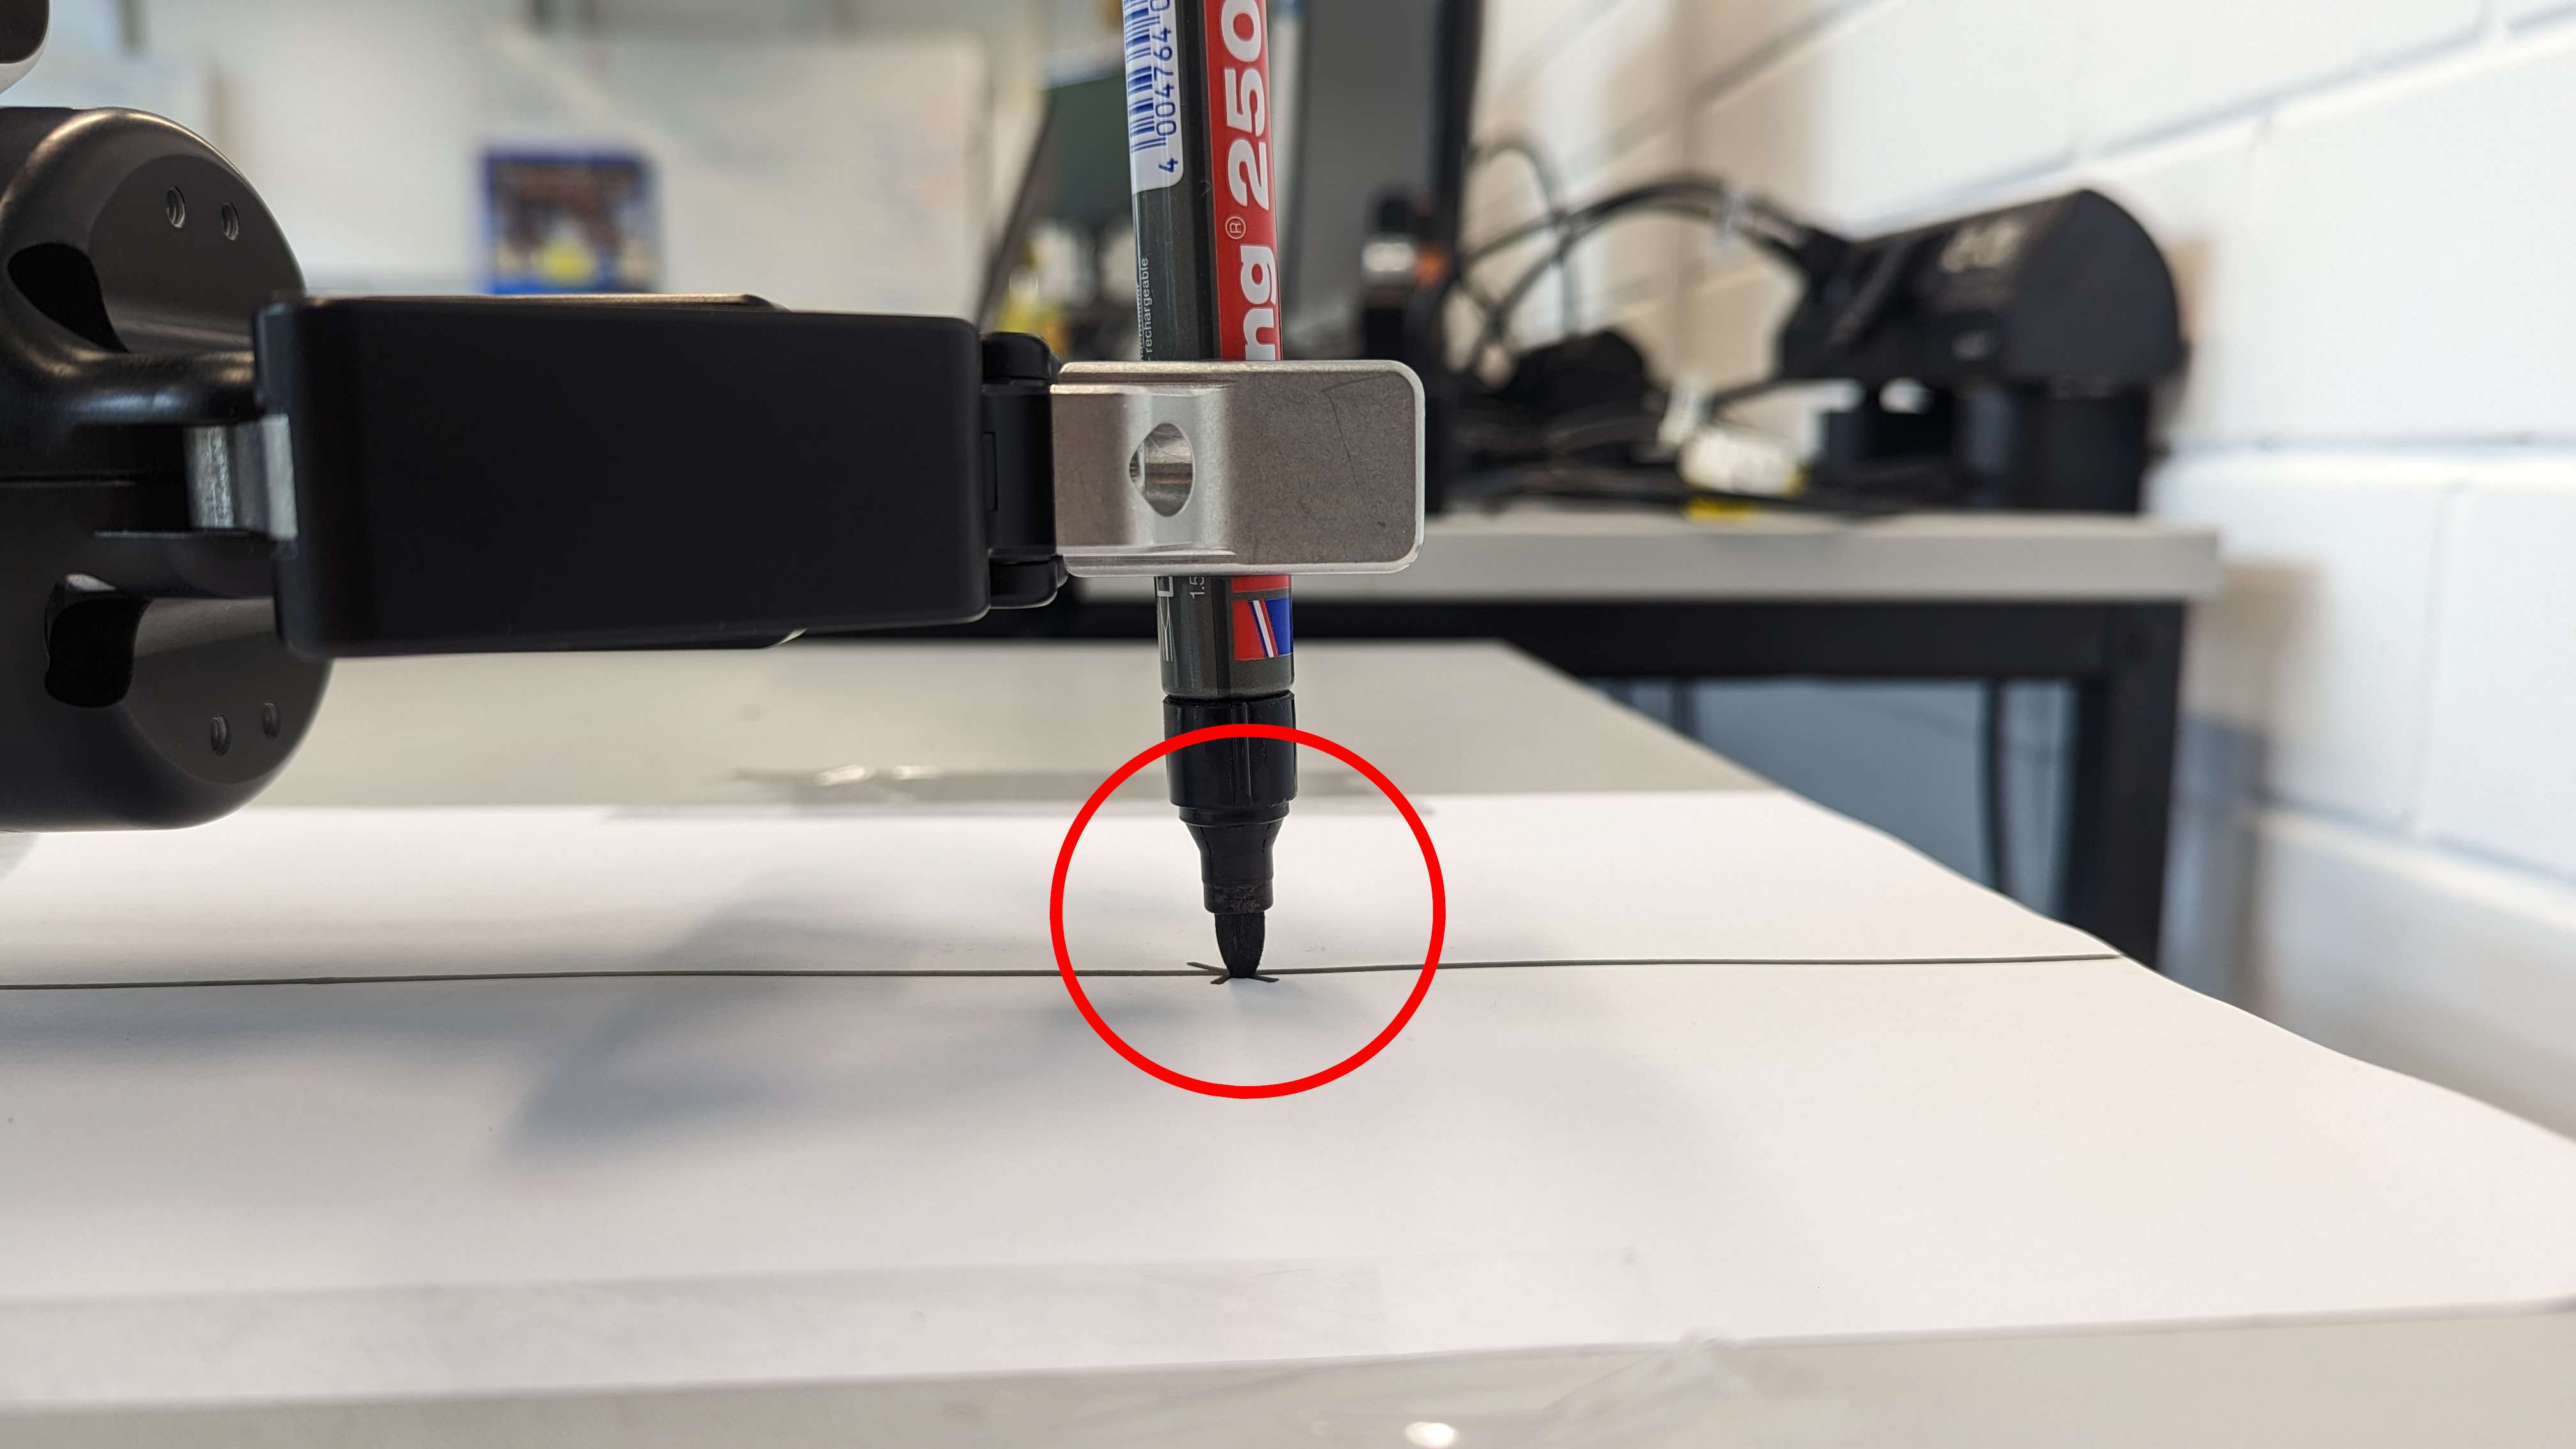
\includegraphics[width=0.8\linewidth]{images/us2_starting_circle.jpg}
        \caption{The tip of the marker pen touches the starting reference point, indicates the robot arm is at the stating position}
        \label{fig:us2_pen}
    \end{figure}
    \begin{figure}[H]
    \captionsetup[subfigure]{justification=centering}
    \begin{subfigure}{0.5\textwidth}
            \centering
            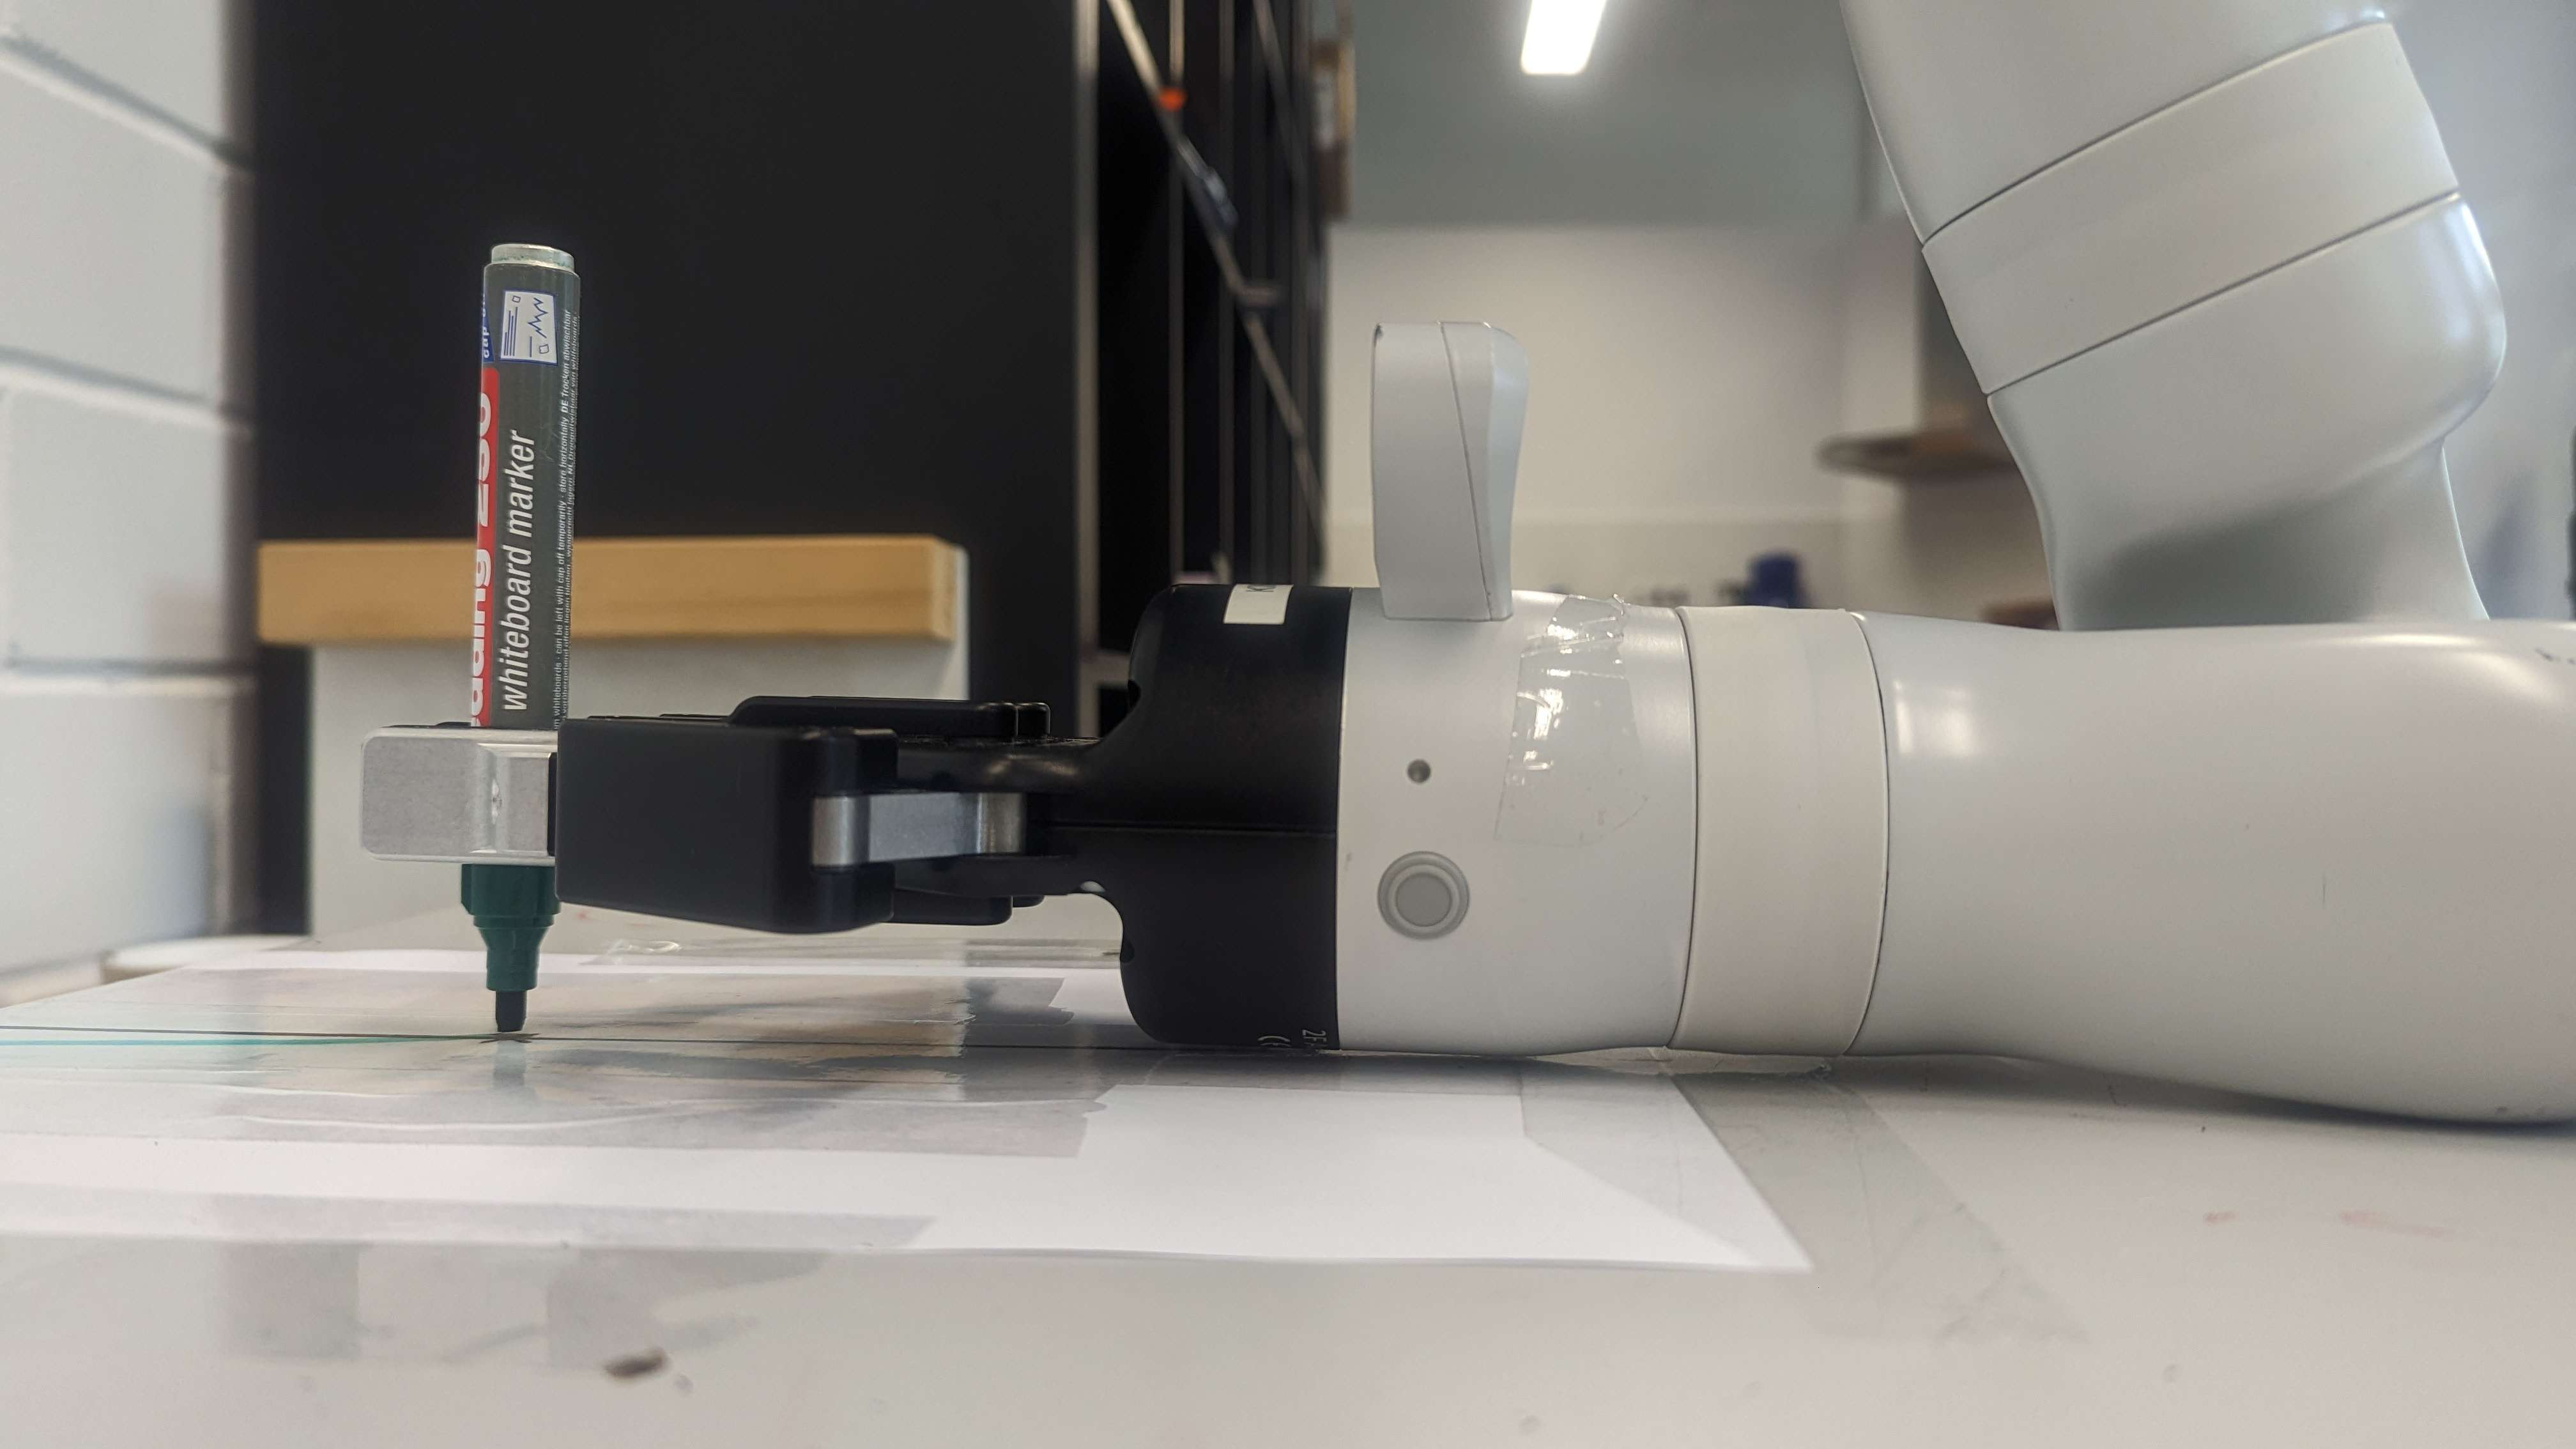
\includegraphics[width=\linewidth]{images/us2_contact.jpg}
            \caption{The initial pose of the robot arm of use case 2 in contact condition}
            \label{fig:us2_init_con}
        \end{subfigure}
        \begin{subfigure}{0.5\textwidth}
            \centering
            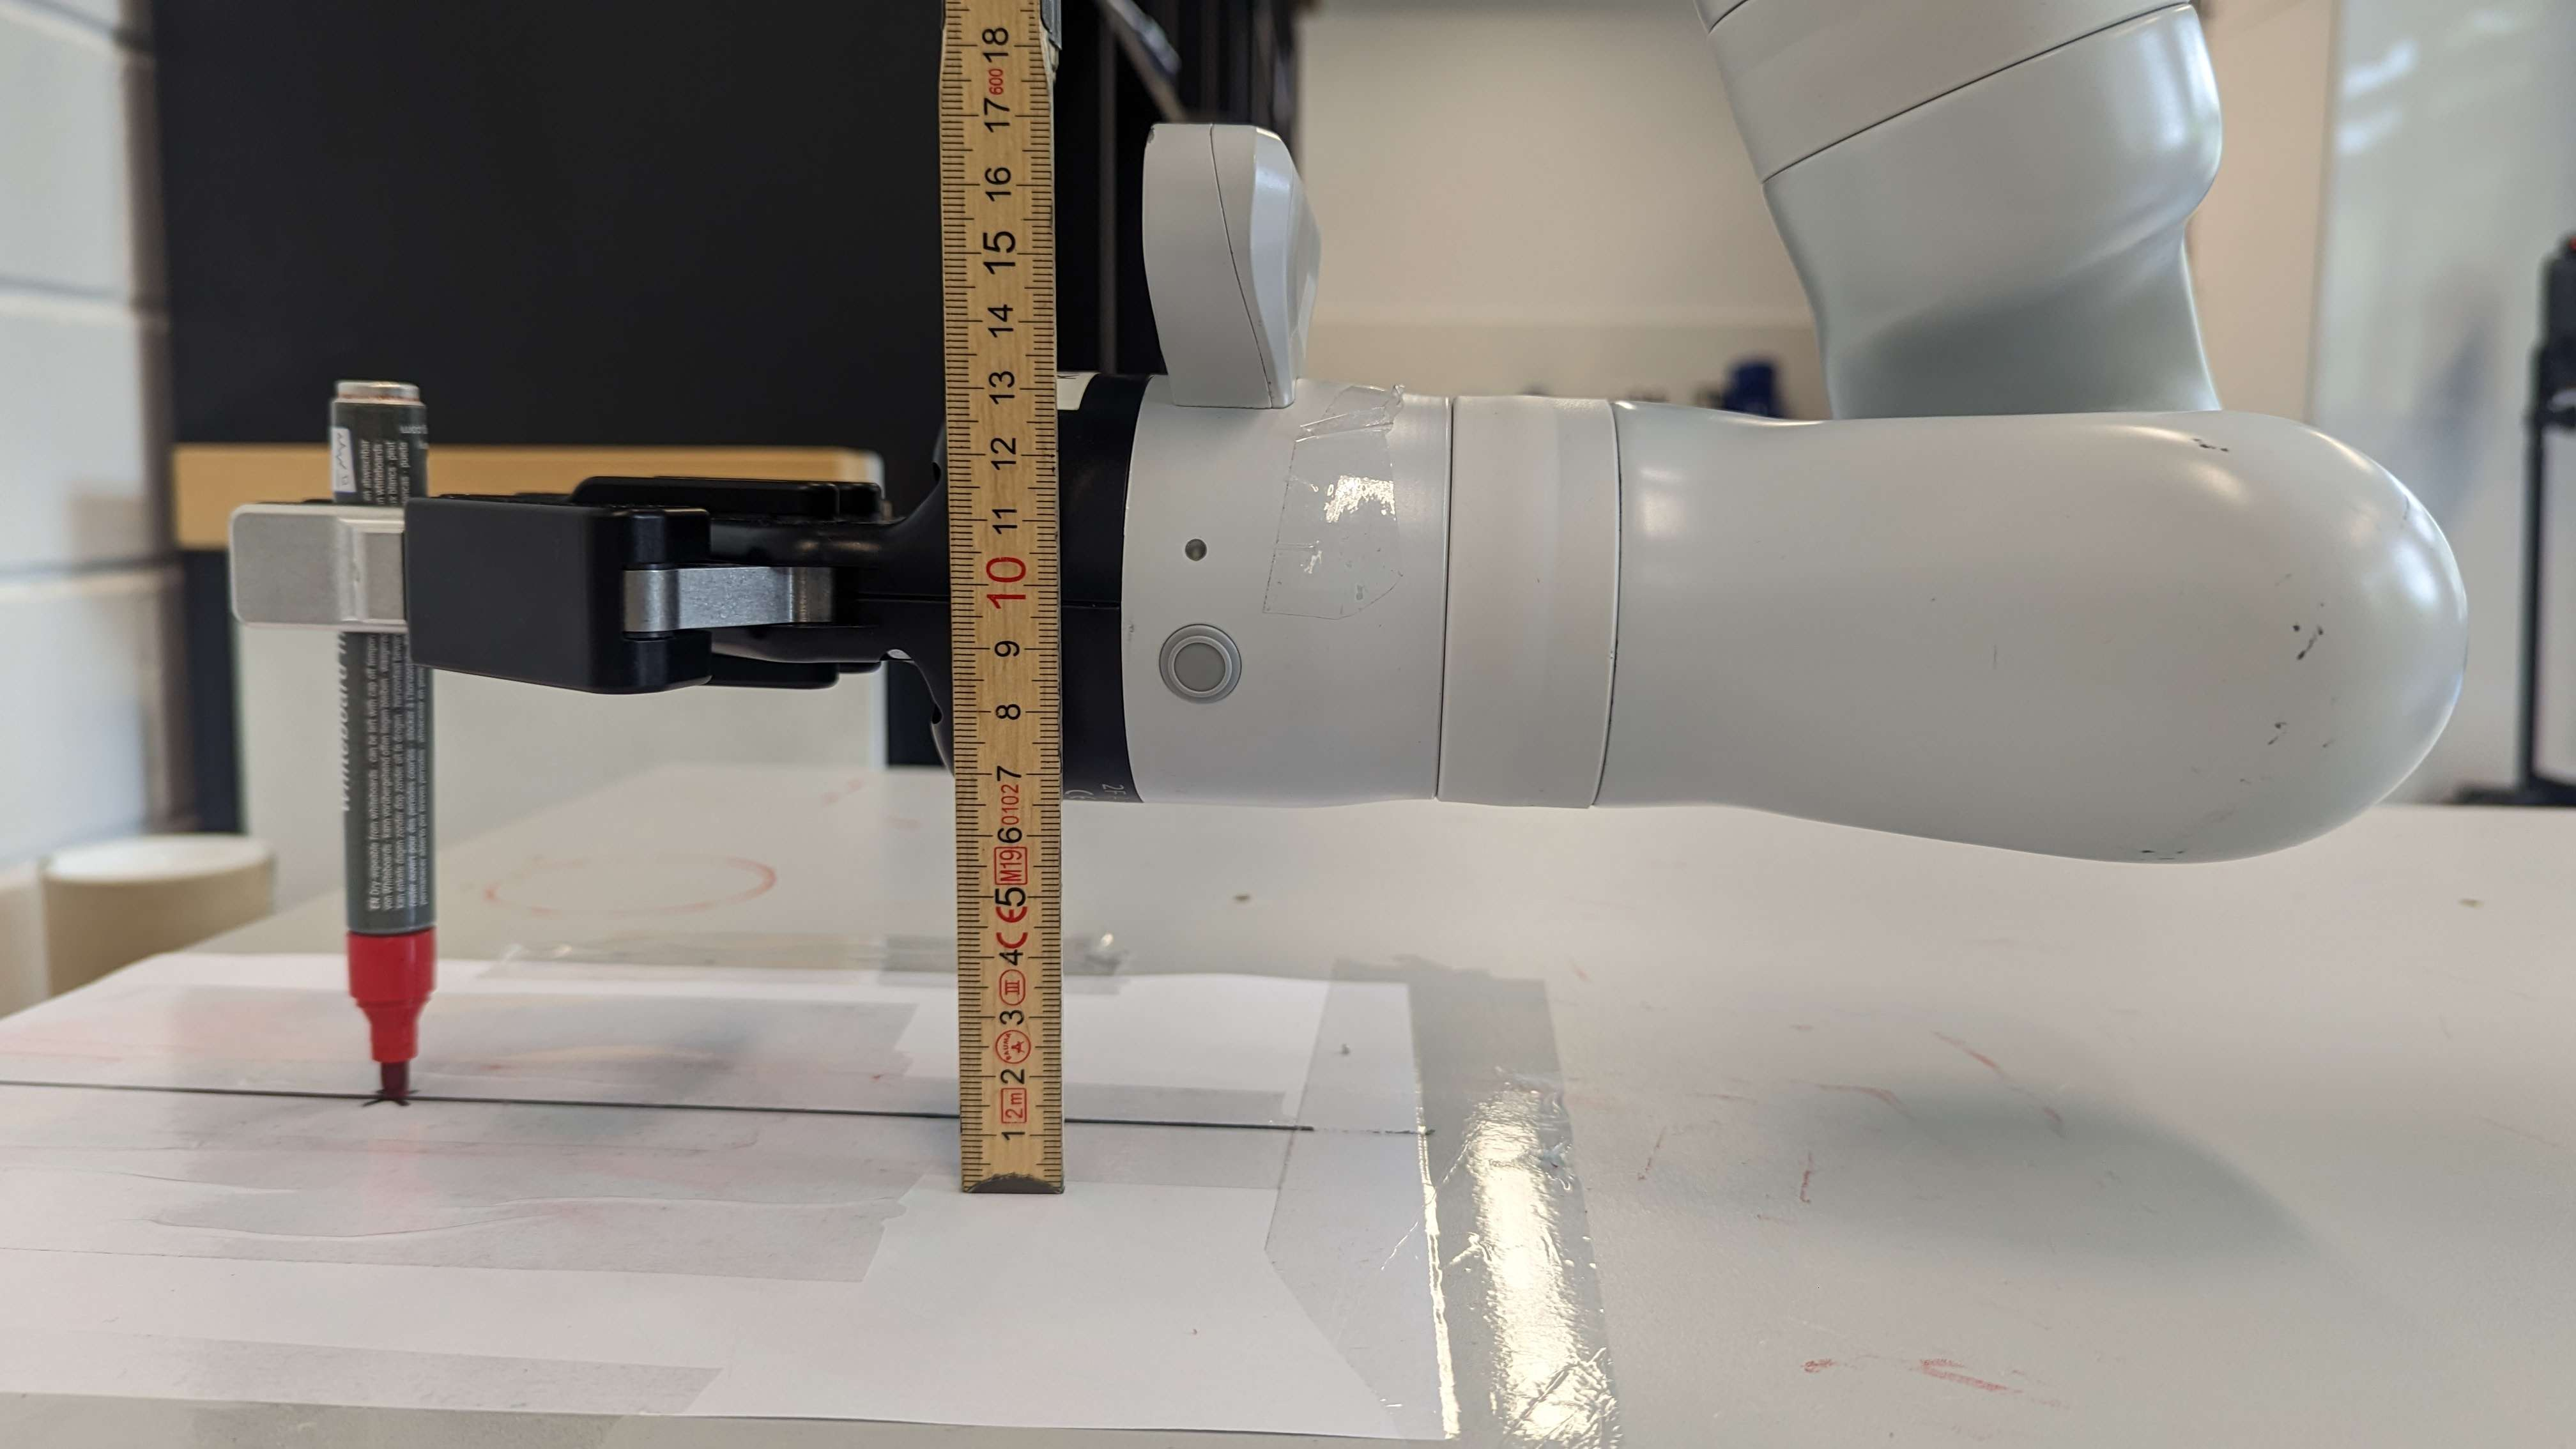
\includegraphics[width=\linewidth]{images/us2_nocontact.jpg}
            \caption{The initial pose of the robot arm of use case 2 in contactless condition}
            \label{fig:us2_init_nocon}
        \end{subfigure}
        \caption{Initial positions of use case 2}
    \end{figure}
    \paragraph{\large{Evaluation}\\}
    The plots below depict the robot's trajectory with and without contact with the table. In the contact case, as shown in Figure \ref{fig:us2_con_plot}, the trajectory exhibits misalignment with the reference line at the start of motion, and the displacement between the measured trajectory and the reference trajectory continues to increase.
    In contrast, Figure \ref{fig:us2_nocon_plot} illustrates the situation in the contactless scenario, where the measured trajectory closely follows the reference trajectory until approximately 0.42 meters, after which it starts to deviate. When we compare both trajectories in Figure \ref{fig:us2_traj_com_plot}, we observe distinct motion behaviors between the two cases.
    In the contact case, the motion appears less stable as indicated by the less smooth trajectory, possibly due to friction on the contact surface. Table \ref{tab:us2_displacement} further supports this observation, revealing that the maximum displacements in the contact case are significantly larger than those in the contactless situation, and the absolute average displacements 4 times in the contactless case.
    This indicates that when the robot arm makes contact with a surface for support in the linear z-direction, considering accuracy based on the average displacement comparison, opting for contactless manipulation of the robot could be viewed as an optimal choice. This observation is unexpected and contradicts the hypothesis of use case 2. This could be attributed to the situation where the constraint on the linear z-direction is removed, leaving the motion subject to the influence of natural forces like gravity. However, the robot must still exert partial control over other directions to ensure that the end effector moves along the x-axis, albeit with greater friction compared to a contactless scenario. During this sliding motion, the end effector might inadvertently shift along the linear x and y axes or even undergo rotation as it attempts to overcome the friction between itself and the contact surface. Given that the surface is not entirely flat, these dynamics may introduce disturbances in various directions of motion.
    \begin{figure}[H]
        \captionsetup[figure]{justification=centering}
                \centering
                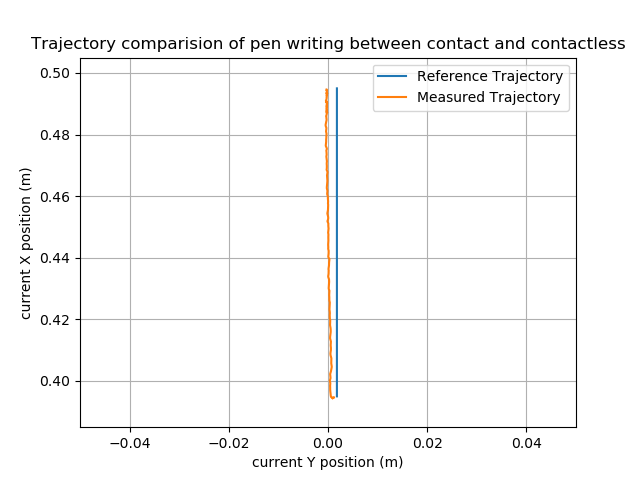
\includegraphics[width=0.8\linewidth]{images/us2_contact_traj.png}
                \caption{The trajectory of pen writing in contact case}
                \label{fig:us2_con_plot}
            \end{figure}

    \begin{figure}[H]
        \captionsetup[figure]{justification=centering}
                \centering
                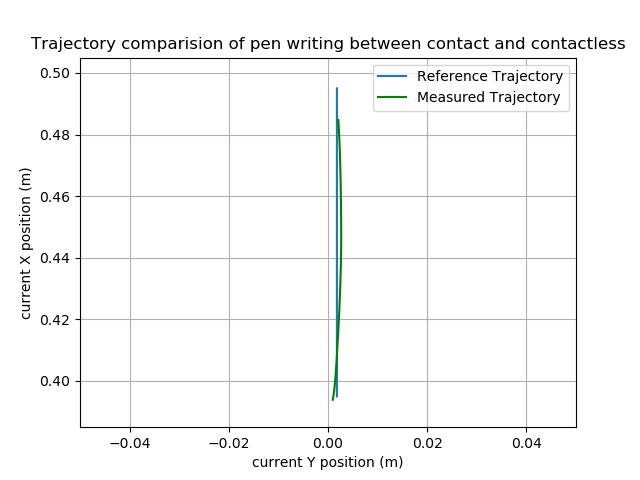
\includegraphics[width=0.8\linewidth]{images/us2_contactless_traj.png}
                \caption{The trajectory of pen writing in contactless case}
                \label{fig:us2_nocon_plot}
    \end{figure}
    \begin{figure}[H]
        \centering
        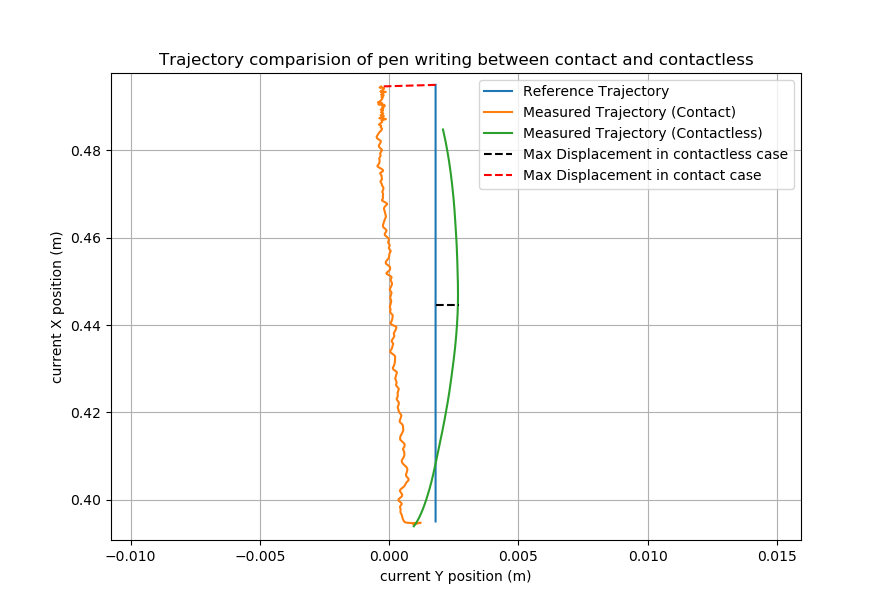
\includegraphics[width=\linewidth]{images/us2_contactless_traj2.png}
        \caption{Trajectory comparision of writing task between contact and contactless}
        \label{fig:us2_traj_com_plot}
\end{figure}
\begin{figure}[H]
    \captionsetup[figure]{justification=centering}
    \centering
    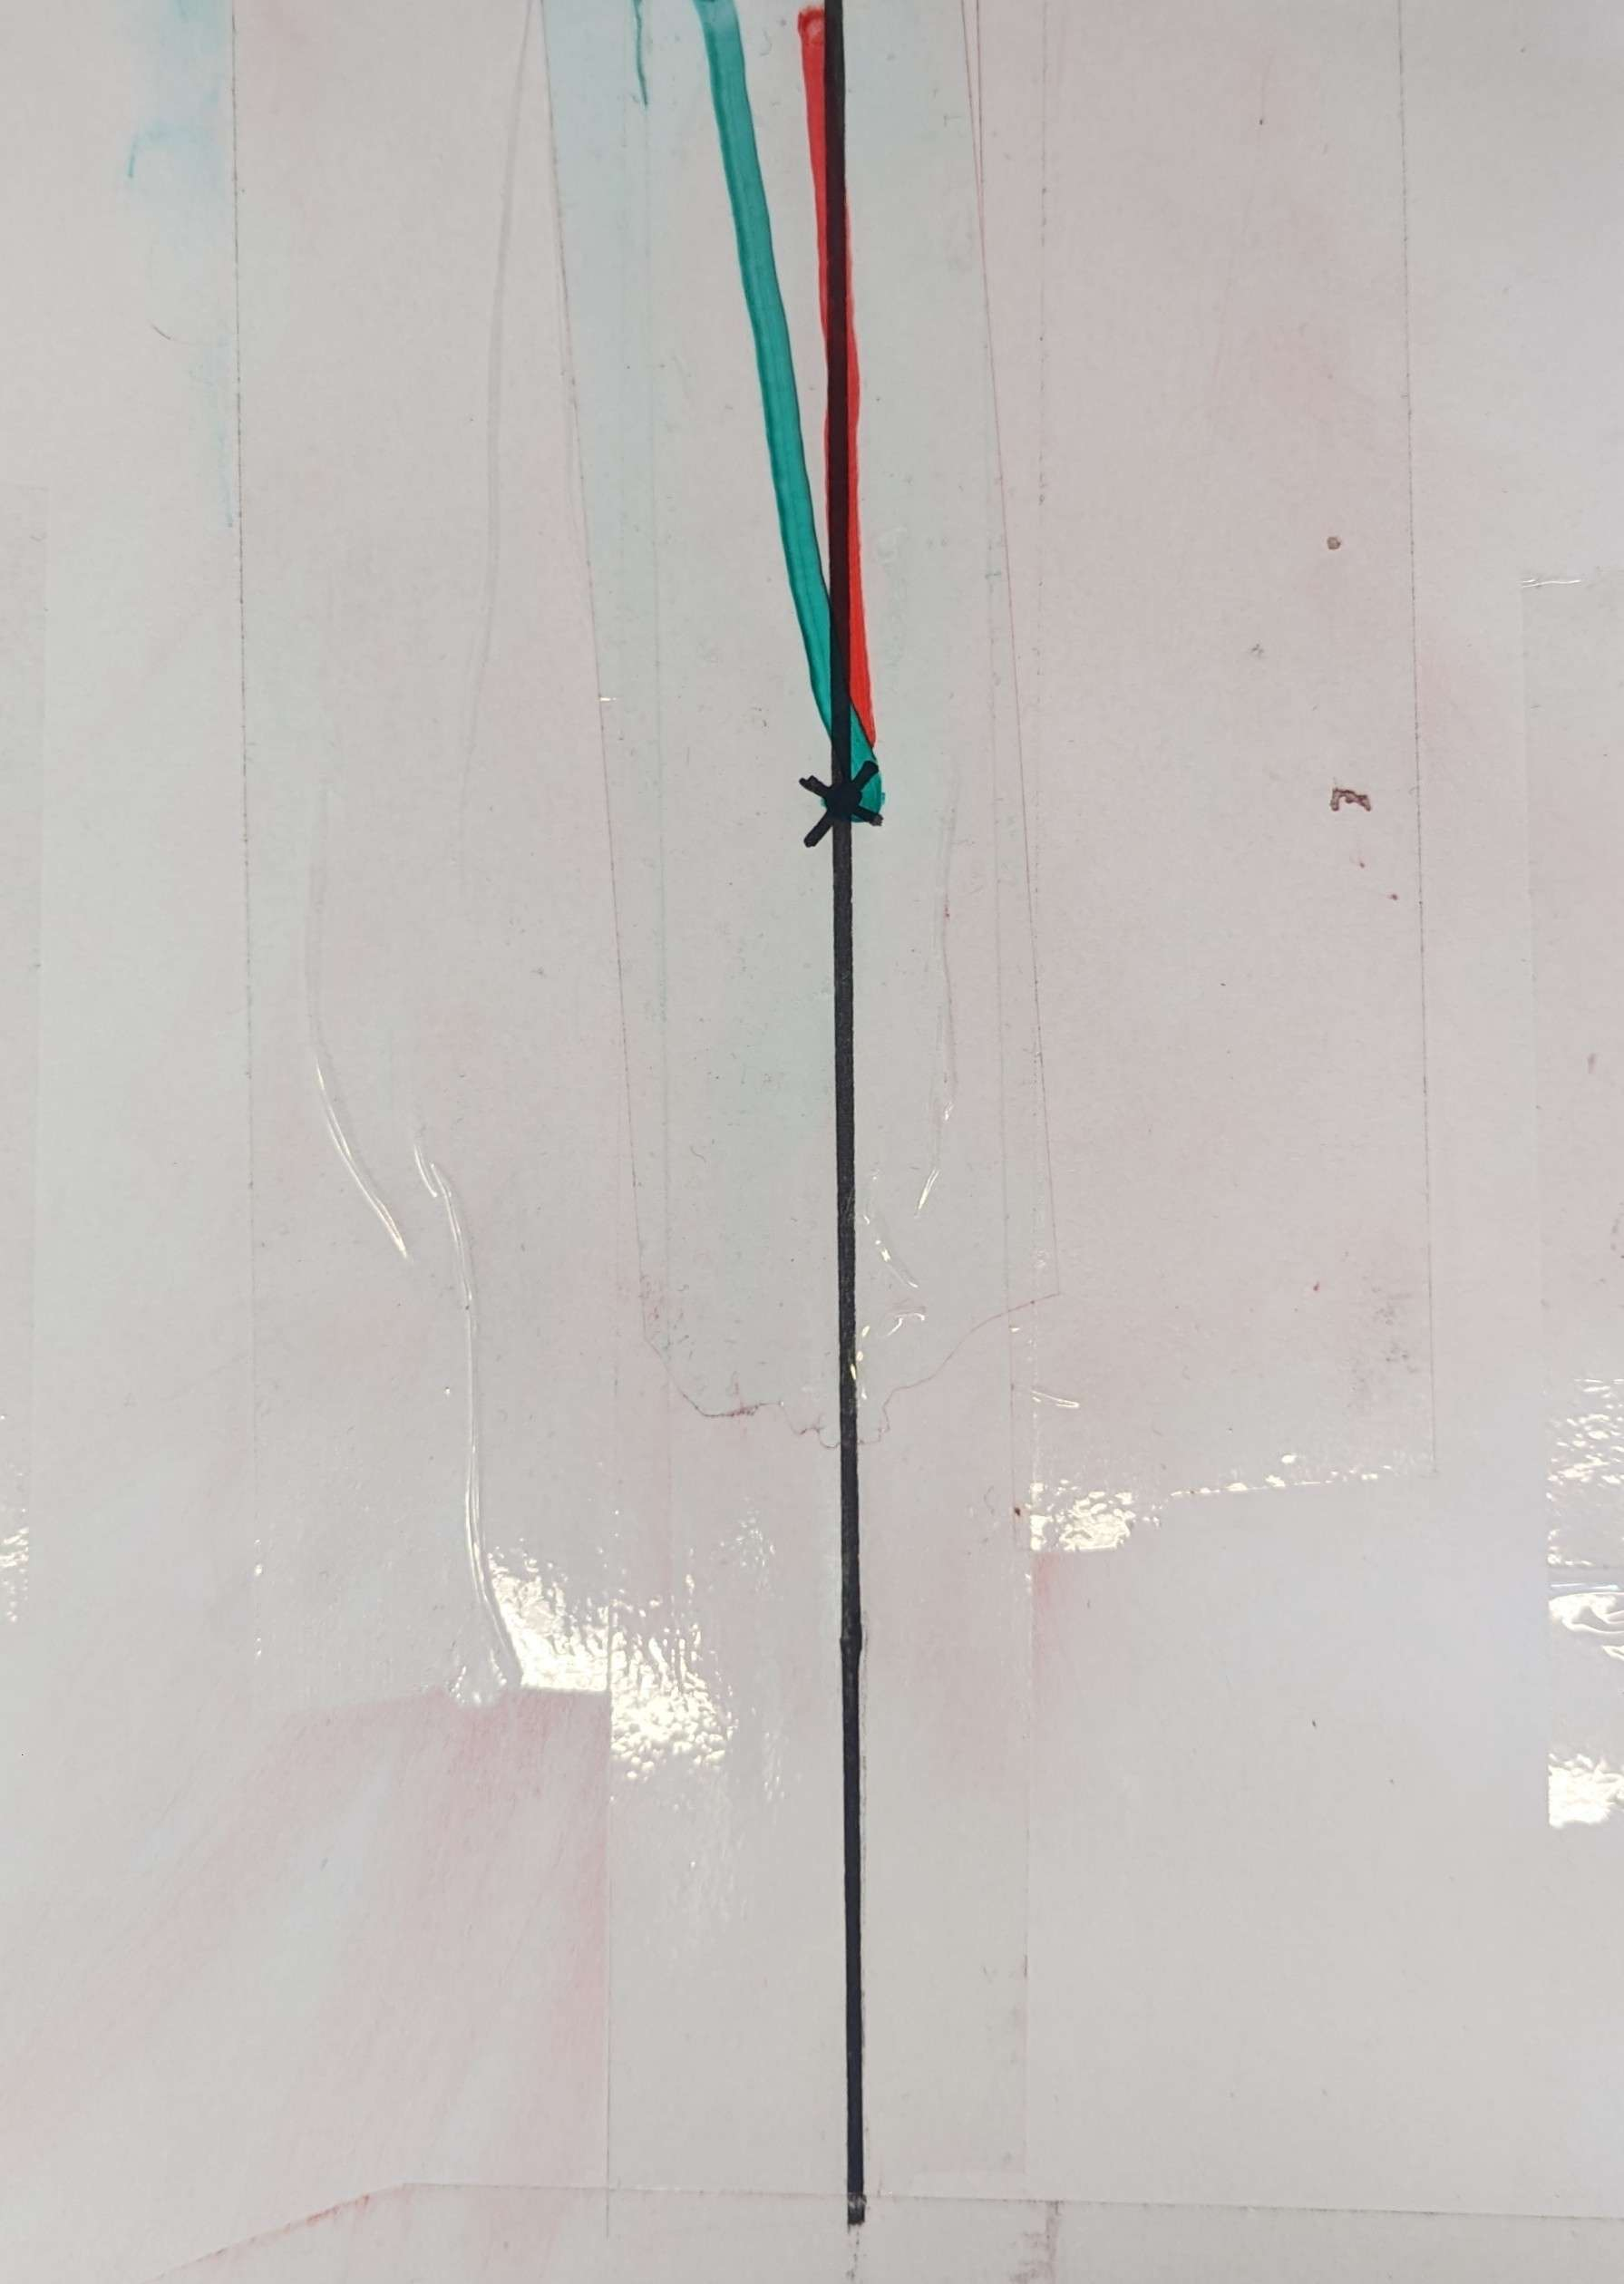
\includegraphics[width=0.5\linewidth]{images/us2_real_compare.jpg}
    \caption{The actual trajectory comparision of writing task between contact and contactless.\\Green line: contact case. Red line: contactless case}
    \label{fig:us2_traj_com_real}
\end{figure}
\begin{table}[H]
    \centering
    % \resizebox{\textwidth}{!}{%
    \begin{tabular}{c|c|c|}
    \cline{2-3}
                                      & maximum displacements(m) & average displacements(m) \\ \hline
    \multicolumn{1}{|c|}{Contact}     &  0.00211145              & -0.00120878               \\ \hline
    \multicolumn{1}{|c|}{Contactless} &  0.00089509              &  0.00034292              \\ \hline
    \end{tabular}%
    % }
    \caption{Table of the average displacement, and maximum displacement in contact and contactless case}
    \label{tab:us2_displacement}
    \end{table}

\newpage
\section{Use case 3 - Resting elbow manipulation}
    \paragraph{\larger{Experiment design}\\}
    The objective of this use case is to assess the potential increase in energy efficiency by allowing certain joints of the manipulator to rest on a supporting surface. The manipulator will execute a standardized task, such as graspung object and writing tasks, under two different conditions: one with the joints resting on a surface (e.g., elbows) and another with the joints suspended in midair. The study will involve a comparison of energy consumption during the execution of the same task under these two conditions to determine if resting joints on a surface leads to improved energy efficiency. The hypothesis of use case is that the energy efficiency will be higher as use case 1 demostrates.
    \paragraph{\large{Setup}\\}
    In this use case, the robot's elbow joint is positioned atop a book, simulating the way humans rest their elbows on a surface when performing tasks such as picking up objects or writing. Figure \ref{fig:us3_init} demostrates the robot set up at a top view.
    \begin{figure}[H]
        \captionsetup[subfigure]{justification=centering}
        \begin{subfigure}{0.5\textwidth}
        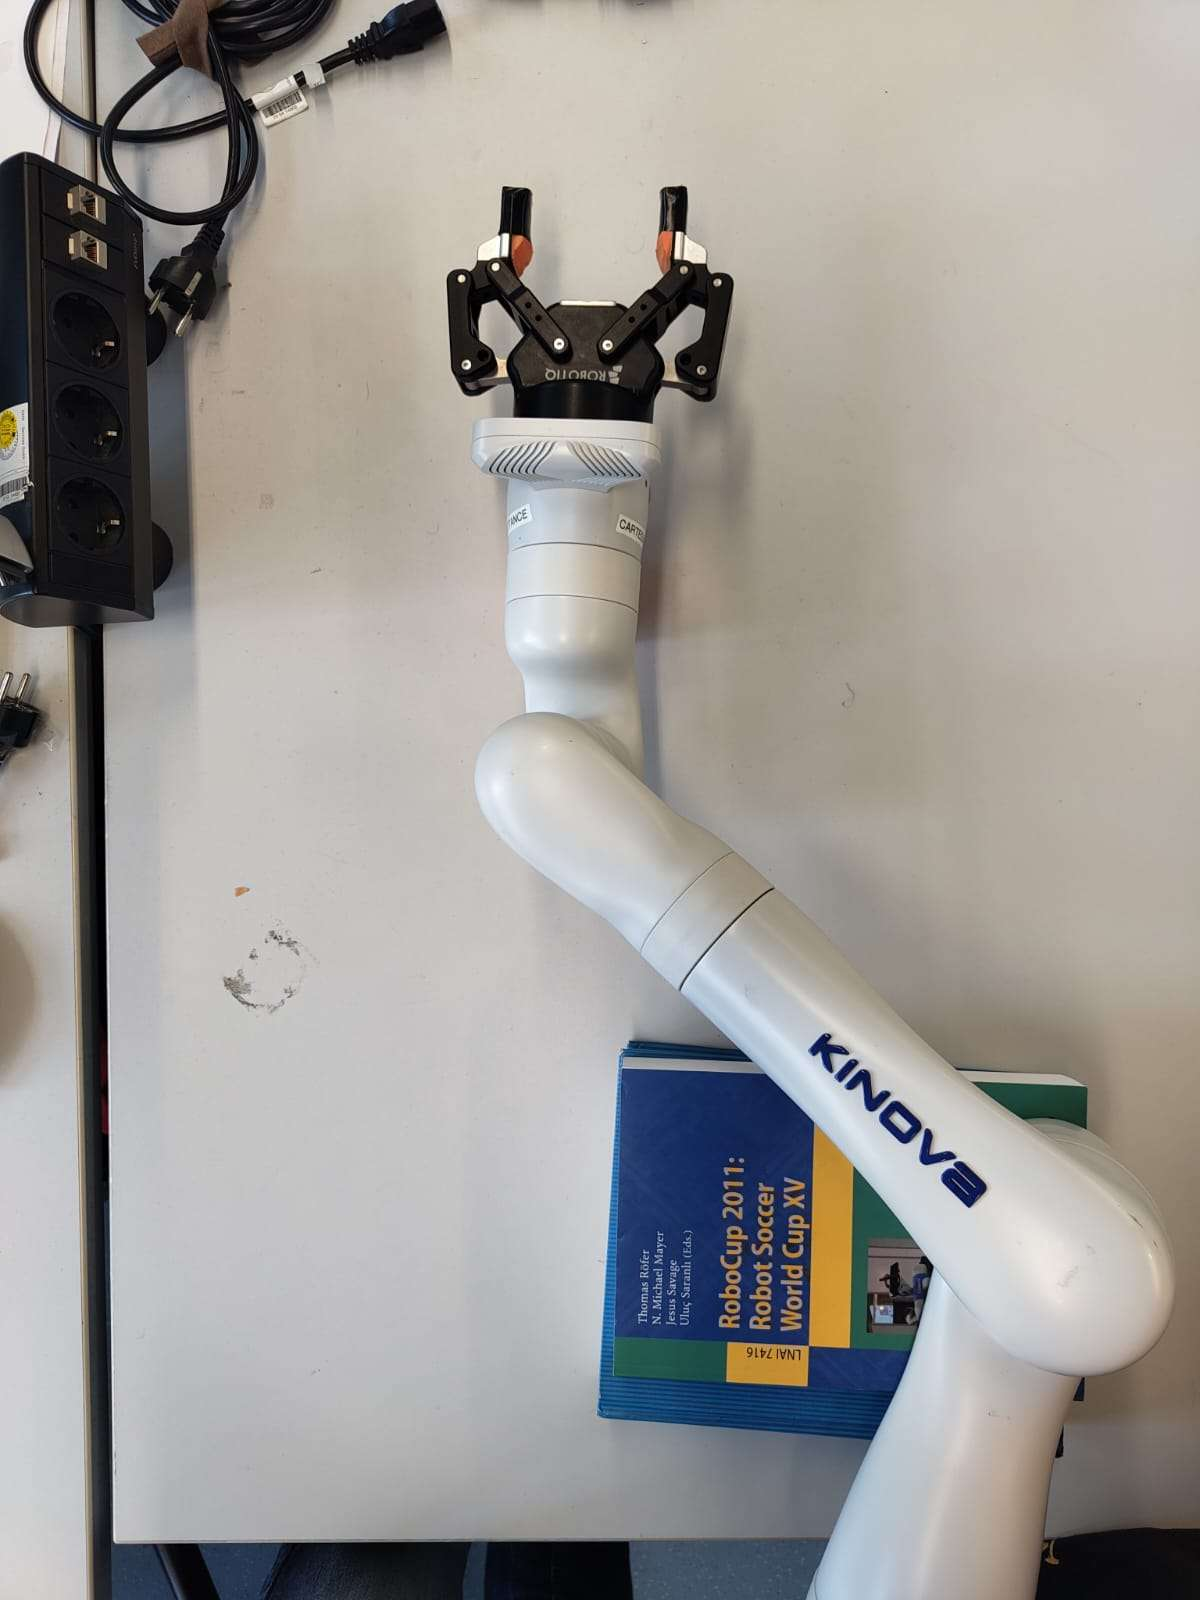
\includegraphics[width=\linewidth]{images/us3_initial.jpg}
        \caption{The initial position of the robot arm in use case 3 where the elbow joint is resting on a book}
        \label{fig:us3_init}
    \end{subfigure}
        \begin{subfigure}{0.5\textwidth}
            \centering
            \captionsetup[figure]{justification=centering}
            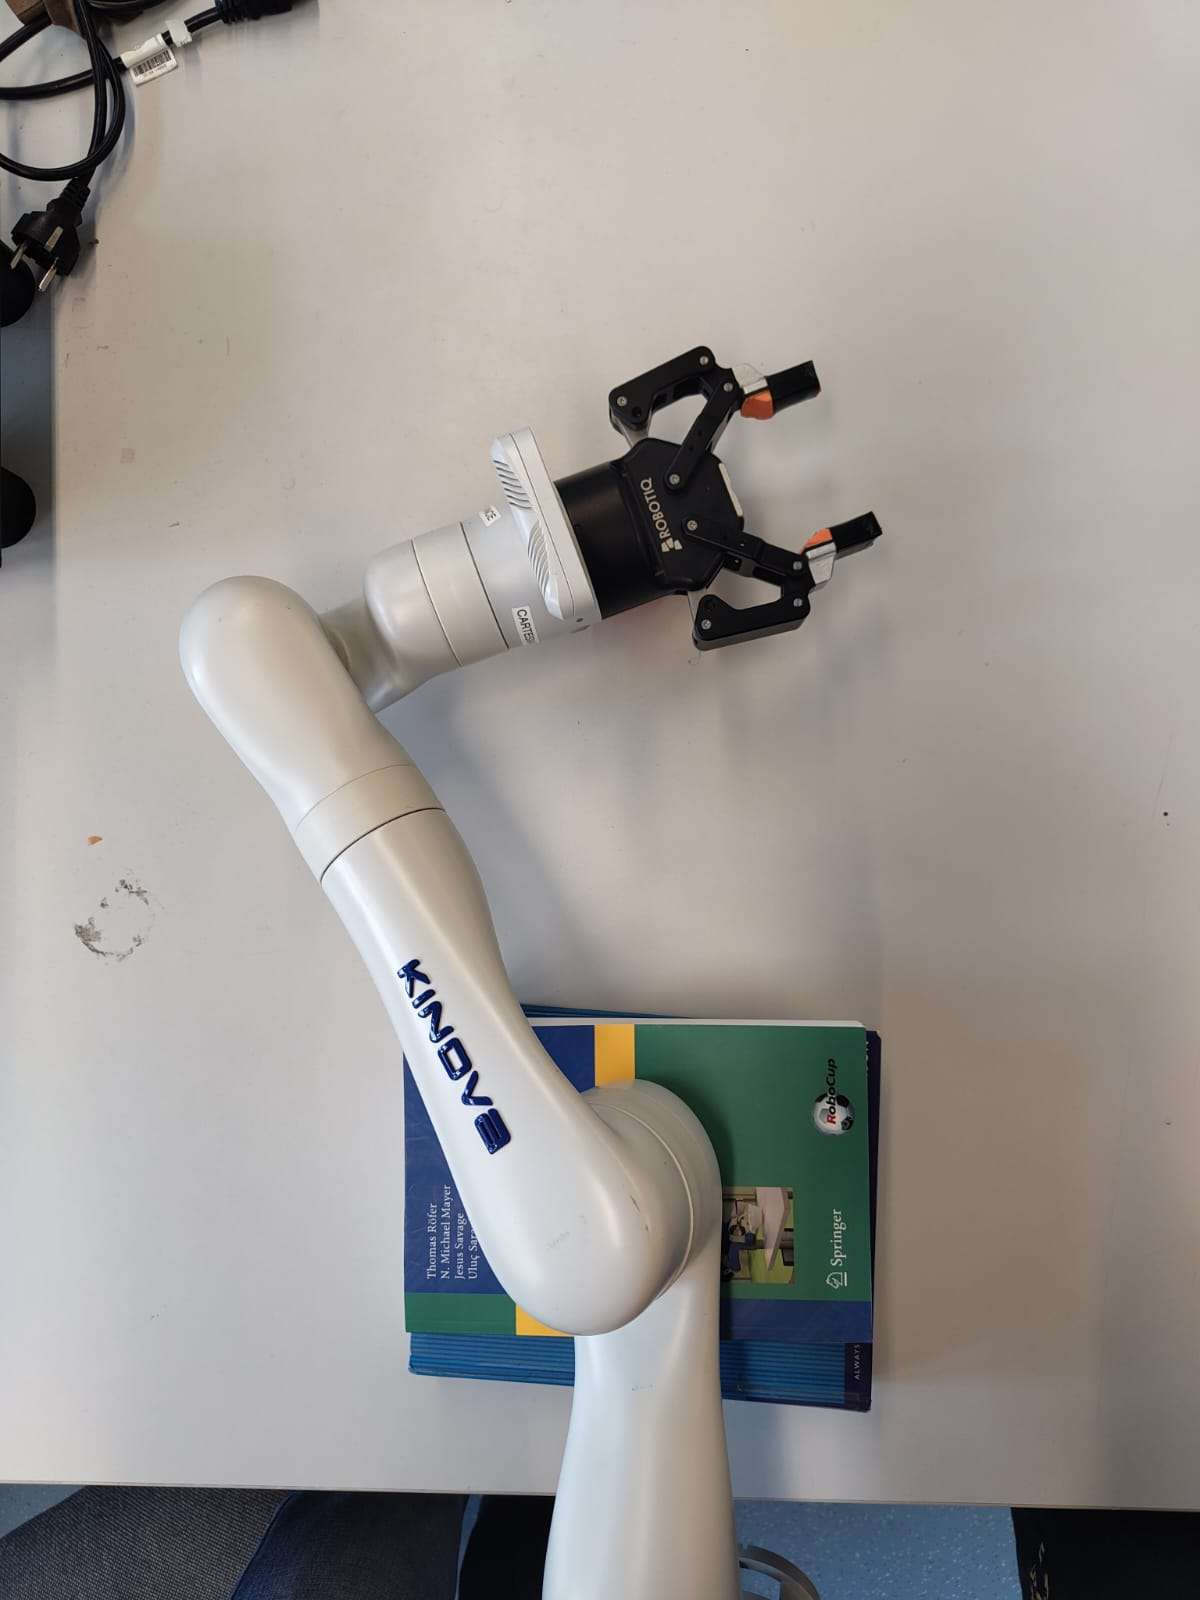
\includegraphics[width=\linewidth]{images/us3_final.jpg}
            \caption{The final position of the robot arm in use case 3 where the elbow joint is resting on a book}
            \label{fig:us3_end}
        \end{subfigure}
        \caption{Robot arm behaviour in use case 2}
    \end{figure}
    \paragraph{\large{Evaluation}\\}
    A difficutie was encountered when conduct the experiement of this use case. As \ref{fig:us3_init} showed the initial position. The elbow joint of the robot manipulator is resting on a stack of book and the constriant on linear z direction is disabled but the constriant on the other direction in enabled such that the robot will not rotate and perform grasping task as use case 1. However, when the robot starts the motion, the 6th joint started to rotate in clockwise direction where in the program, the acceleration energy of angular z is being controlled by the cascaded controller where the set point is equals to zero. Means the controller is maintaining zero acceleration energy in angular z direction and joint 6 should not rotate as in figure \ref{fig:us3_end} shows. The hypothesis of such behaviour could be the P gains (linear and angular) is not high enough so the end effector cannot rotate back to the set point orientation on time. As the rotational motion led to the 6th joint reaching its limit and subsequently resulted in the termination of the program, the experiment was unable to proceed further. However, it is worth considering that in future attempts, fine-tuning the P gains settings might offer a potential solution for enhancing the motion.
    % \begin{figure}[H]
    %     \centering
    %     \captionsetup[figure]{justification=centering}
    %     \includegraphics[width=0.5\linewidth]{images/us3_}
    %     \caption{The initial position of the robot arm in use case 3 where the elbow joint is resting on a book}
    %     \label{fig:us3_init}
    % \end{figure}
\end{document}
